% Options for packages loaded elsewhere
\PassOptionsToPackage{unicode}{hyperref}
\PassOptionsToPackage{hyphens}{url}
\PassOptionsToPackage{dvipsnames,svgnames,x11names}{xcolor}
%
\documentclass[
  letterpaper,
  DIV=11,
  numbers=noendperiod]{scrartcl}

\usepackage{amsmath,amssymb}
\usepackage{lmodern}
\usepackage{iftex}
\ifPDFTeX
  \usepackage[T1]{fontenc}
  \usepackage[utf8]{inputenc}
  \usepackage{textcomp} % provide euro and other symbols
\else % if luatex or xetex
  \usepackage{unicode-math}
  \defaultfontfeatures{Scale=MatchLowercase}
  \defaultfontfeatures[\rmfamily]{Ligatures=TeX,Scale=1}
\fi
% Use upquote if available, for straight quotes in verbatim environments
\IfFileExists{upquote.sty}{\usepackage{upquote}}{}
\IfFileExists{microtype.sty}{% use microtype if available
  \usepackage[]{microtype}
  \UseMicrotypeSet[protrusion]{basicmath} % disable protrusion for tt fonts
}{}
\makeatletter
\@ifundefined{KOMAClassName}{% if non-KOMA class
  \IfFileExists{parskip.sty}{%
    \usepackage{parskip}
  }{% else
    \setlength{\parindent}{0pt}
    \setlength{\parskip}{6pt plus 2pt minus 1pt}}
}{% if KOMA class
  \KOMAoptions{parskip=half}}
\makeatother
\usepackage{xcolor}
\setlength{\emergencystretch}{3em} % prevent overfull lines
\setcounter{secnumdepth}{1}
% Make \paragraph and \subparagraph free-standing
\ifx\paragraph\undefined\else
  \let\oldparagraph\paragraph
  \renewcommand{\paragraph}[1]{\oldparagraph{#1}\mbox{}}
\fi
\ifx\subparagraph\undefined\else
  \let\oldsubparagraph\subparagraph
  \renewcommand{\subparagraph}[1]{\oldsubparagraph{#1}\mbox{}}
\fi

\usepackage{color}
\usepackage{fancyvrb}
\newcommand{\VerbBar}{|}
\newcommand{\VERB}{\Verb[commandchars=\\\{\}]}
\DefineVerbatimEnvironment{Highlighting}{Verbatim}{commandchars=\\\{\}}
% Add ',fontsize=\small' for more characters per line
\usepackage{framed}
\definecolor{shadecolor}{RGB}{241,243,245}
\newenvironment{Shaded}{\begin{snugshade}}{\end{snugshade}}
\newcommand{\AlertTok}[1]{\textcolor[rgb]{0.68,0.00,0.00}{#1}}
\newcommand{\AnnotationTok}[1]{\textcolor[rgb]{0.37,0.37,0.37}{#1}}
\newcommand{\AttributeTok}[1]{\textcolor[rgb]{0.40,0.45,0.13}{#1}}
\newcommand{\BaseNTok}[1]{\textcolor[rgb]{0.68,0.00,0.00}{#1}}
\newcommand{\BuiltInTok}[1]{\textcolor[rgb]{0.00,0.23,0.31}{#1}}
\newcommand{\CharTok}[1]{\textcolor[rgb]{0.13,0.47,0.30}{#1}}
\newcommand{\CommentTok}[1]{\textcolor[rgb]{0.37,0.37,0.37}{#1}}
\newcommand{\CommentVarTok}[1]{\textcolor[rgb]{0.37,0.37,0.37}{\textit{#1}}}
\newcommand{\ConstantTok}[1]{\textcolor[rgb]{0.56,0.35,0.01}{#1}}
\newcommand{\ControlFlowTok}[1]{\textcolor[rgb]{0.00,0.23,0.31}{#1}}
\newcommand{\DataTypeTok}[1]{\textcolor[rgb]{0.68,0.00,0.00}{#1}}
\newcommand{\DecValTok}[1]{\textcolor[rgb]{0.68,0.00,0.00}{#1}}
\newcommand{\DocumentationTok}[1]{\textcolor[rgb]{0.37,0.37,0.37}{\textit{#1}}}
\newcommand{\ErrorTok}[1]{\textcolor[rgb]{0.68,0.00,0.00}{#1}}
\newcommand{\ExtensionTok}[1]{\textcolor[rgb]{0.00,0.23,0.31}{#1}}
\newcommand{\FloatTok}[1]{\textcolor[rgb]{0.68,0.00,0.00}{#1}}
\newcommand{\FunctionTok}[1]{\textcolor[rgb]{0.28,0.35,0.67}{#1}}
\newcommand{\ImportTok}[1]{\textcolor[rgb]{0.00,0.46,0.62}{#1}}
\newcommand{\InformationTok}[1]{\textcolor[rgb]{0.37,0.37,0.37}{#1}}
\newcommand{\KeywordTok}[1]{\textcolor[rgb]{0.00,0.23,0.31}{#1}}
\newcommand{\NormalTok}[1]{\textcolor[rgb]{0.00,0.23,0.31}{#1}}
\newcommand{\OperatorTok}[1]{\textcolor[rgb]{0.37,0.37,0.37}{#1}}
\newcommand{\OtherTok}[1]{\textcolor[rgb]{0.00,0.23,0.31}{#1}}
\newcommand{\PreprocessorTok}[1]{\textcolor[rgb]{0.68,0.00,0.00}{#1}}
\newcommand{\RegionMarkerTok}[1]{\textcolor[rgb]{0.00,0.23,0.31}{#1}}
\newcommand{\SpecialCharTok}[1]{\textcolor[rgb]{0.37,0.37,0.37}{#1}}
\newcommand{\SpecialStringTok}[1]{\textcolor[rgb]{0.13,0.47,0.30}{#1}}
\newcommand{\StringTok}[1]{\textcolor[rgb]{0.13,0.47,0.30}{#1}}
\newcommand{\VariableTok}[1]{\textcolor[rgb]{0.07,0.07,0.07}{#1}}
\newcommand{\VerbatimStringTok}[1]{\textcolor[rgb]{0.13,0.47,0.30}{#1}}
\newcommand{\WarningTok}[1]{\textcolor[rgb]{0.37,0.37,0.37}{\textit{#1}}}

\providecommand{\tightlist}{%
  \setlength{\itemsep}{0pt}\setlength{\parskip}{0pt}}\usepackage{longtable,booktabs,array}
\usepackage{calc} % for calculating minipage widths
% Correct order of tables after \paragraph or \subparagraph
\usepackage{etoolbox}
\makeatletter
\patchcmd\longtable{\par}{\if@noskipsec\mbox{}\fi\par}{}{}
\makeatother
% Allow footnotes in longtable head/foot
\IfFileExists{footnotehyper.sty}{\usepackage{footnotehyper}}{\usepackage{footnote}}
\makesavenoteenv{longtable}
\usepackage{graphicx}
\makeatletter
\def\maxwidth{\ifdim\Gin@nat@width>\linewidth\linewidth\else\Gin@nat@width\fi}
\def\maxheight{\ifdim\Gin@nat@height>\textheight\textheight\else\Gin@nat@height\fi}
\makeatother
% Scale images if necessary, so that they will not overflow the page
% margins by default, and it is still possible to overwrite the defaults
% using explicit options in \includegraphics[width, height, ...]{}
\setkeys{Gin}{width=\maxwidth,height=\maxheight,keepaspectratio}
% Set default figure placement to htbp
\makeatletter
\def\fps@figure{htbp}
\makeatother

\KOMAoption{captions}{tableheading}
\makeatletter
\makeatother
\makeatletter
\makeatother
\makeatletter
\@ifpackageloaded{caption}{}{\usepackage{caption}}
\AtBeginDocument{%
\ifdefined\contentsname
  \renewcommand*\contentsname{Table of contents}
\else
  \newcommand\contentsname{Table of contents}
\fi
\ifdefined\listfigurename
  \renewcommand*\listfigurename{List of Figures}
\else
  \newcommand\listfigurename{List of Figures}
\fi
\ifdefined\listtablename
  \renewcommand*\listtablename{List of Tables}
\else
  \newcommand\listtablename{List of Tables}
\fi
\ifdefined\figurename
  \renewcommand*\figurename{Figure}
\else
  \newcommand\figurename{Figure}
\fi
\ifdefined\tablename
  \renewcommand*\tablename{Table}
\else
  \newcommand\tablename{Table}
\fi
}
\@ifpackageloaded{float}{}{\usepackage{float}}
\floatstyle{ruled}
\@ifundefined{c@chapter}{\newfloat{codelisting}{h}{lop}}{\newfloat{codelisting}{h}{lop}[chapter]}
\floatname{codelisting}{Listing}
\newcommand*\listoflistings{\listof{codelisting}{List of Listings}}
\makeatother
\makeatletter
\@ifpackageloaded{caption}{}{\usepackage{caption}}
\@ifpackageloaded{subcaption}{}{\usepackage{subcaption}}
\makeatother
\makeatletter
\@ifpackageloaded{tcolorbox}{}{\usepackage[many]{tcolorbox}}
\makeatother
\makeatletter
\@ifundefined{shadecolor}{\definecolor{shadecolor}{rgb}{.97, .97, .97}}
\makeatother
\makeatletter
\makeatother
\ifLuaTeX
  \usepackage{selnolig}  % disable illegal ligatures
\fi
\IfFileExists{bookmark.sty}{\usepackage{bookmark}}{\usepackage{hyperref}}
\IfFileExists{xurl.sty}{\usepackage{xurl}}{} % add URL line breaks if available
\urlstyle{same} % disable monospaced font for URLs
\hypersetup{
  pdftitle={MD\_01\_RR},
  pdfauthor={Xinchen\_Yang},
  colorlinks=true,
  linkcolor={blue},
  filecolor={Maroon},
  citecolor={Blue},
  urlcolor={Blue},
  pdfcreator={LaTeX via pandoc}}

\title{MD\_01\_RR}
\author{Xinchen\_Yang}
\date{}

\begin{document}
\maketitle
\ifdefined\Shaded\renewenvironment{Shaded}{\begin{tcolorbox}[borderline west={3pt}{0pt}{shadecolor}, sharp corners, enhanced, breakable, frame hidden, interior hidden, boxrule=0pt]}{\end{tcolorbox}}\fi

\hypertarget{task-1}{%
\section{task 1}\label{task-1}}

Suits is an American television drama series created by Aaron Korsh,
which premiered on June 23, 2011 on the USA Network. It revolves around
Mike Ross (Patrick J. Adams), who begins working as a law associate for
Harvey Specter (Gabriel Macht), despite never attending law school. The
show focuses on Harvey and Mike managing to close cases, while
maintaining Mike's secret.

The series was renewed for an eighth season on January 30, 2018.{[}1{]}
In January 2019, the series was renewed for a ninth and final season
which premiered on July 17, 2019.{[}2{]} During the course of the
series, 134 episodes of Suits aired over nine seasons, between June 23,
2011, and September 25, 2019.

\hypertarget{task-2}{%
\section{task 2}\label{task-2}}

\begin{figure}

{\centering 
\includegraphics{images/Suits_Logo.png}

}

\caption{suits\_logo}

\end{figure}

\hypertarget{task-3}{%
\section{task 3}\label{task-3}}

\begin{longtable}[]{@{}lcr@{}}
\toprule()
Title & Directed by & U.S. viewers (millions) \\
\midrule()
\endhead
``Pilot'' & Kevin Bray & 4.64 \\
``Errors and Omissions'' & John Scott & 3.89 \\
T ``Inside Track'' & Kevin Bray & 4.53 \\
\bottomrule()
\end{longtable}

\hypertarget{task-4}{%
\section{task 4}\label{task-4}}

\begin{Shaded}
\begin{Highlighting}[]
\FunctionTok{library}\NormalTok{(ggplot2)}

\NormalTok{viewership }\OtherTok{\textless{}{-}} \FunctionTok{c}\NormalTok{(}\FloatTok{4.64}\NormalTok{, }\FloatTok{3.89}\NormalTok{, }\FloatTok{4.53}\NormalTok{, }\FloatTok{4.38}\NormalTok{, }\FloatTok{4.38}\NormalTok{, }\FloatTok{4.44}\NormalTok{, }\FloatTok{4.03}\NormalTok{, }\FloatTok{3.96}\NormalTok{, }\FloatTok{4.45}\NormalTok{, }\FloatTok{3.82}\NormalTok{, }\FloatTok{3.96}\NormalTok{, }\FloatTok{3.47}\NormalTok{, }\FloatTok{3.47}\NormalTok{, }\FloatTok{3.80}\NormalTok{, }\FloatTok{3.88}\NormalTok{, }\FloatTok{3.70}\NormalTok{,}\FloatTok{3.72}\NormalTok{,}\FloatTok{3.89}\NormalTok{,}\FloatTok{3.41}\NormalTok{,}\FloatTok{3.42}\NormalTok{,}\FloatTok{4.00}\NormalTok{,}\FloatTok{4.48}\NormalTok{,}\FloatTok{3.57}\NormalTok{,}\FloatTok{3.75}\NormalTok{,}\FloatTok{3.36}
\NormalTok{                 ,}\FloatTok{3.07}\NormalTok{,}\FloatTok{2.90}\NormalTok{,}\FloatTok{3.20}\NormalTok{,}\FloatTok{2.93}\NormalTok{,}\FloatTok{2.88}\NormalTok{,}\FloatTok{2.47}\NormalTok{,}\FloatTok{2.99}\NormalTok{,}\FloatTok{2.79}\NormalTok{,}\FloatTok{2.76}\NormalTok{,}\FloatTok{2.79}\NormalTok{,}\FloatTok{3.52}\NormalTok{,}\FloatTok{2.95}\NormalTok{,}
                 \FloatTok{3.16}\NormalTok{,}\FloatTok{2.27}\NormalTok{,}\FloatTok{2.27}\NormalTok{,}\FloatTok{2.35}\NormalTok{,}\FloatTok{2.53}\NormalTok{,}\FloatTok{2.50}\NormalTok{,}\FloatTok{2.40}\NormalTok{)}

\NormalTok{df }\OtherTok{\textless{}{-}} \FunctionTok{data.frame}\NormalTok{(}\AttributeTok{x =} \DecValTok{1}\SpecialCharTok{:}\FunctionTok{length}\NormalTok{(viewership), }\AttributeTok{v1 =}\NormalTok{ viewership)}
\FunctionTok{ggplot}\NormalTok{(}\AttributeTok{data =}\NormalTok{ df, }\FunctionTok{aes}\NormalTok{(}\AttributeTok{x =}\NormalTok{ x)) }\SpecialCharTok{+}
  \FunctionTok{geom\_line}\NormalTok{(}\FunctionTok{aes}\NormalTok{(}\AttributeTok{y =}\NormalTok{ v1)) }
\end{Highlighting}
\end{Shaded}

\begin{figure}[H]

{\centering 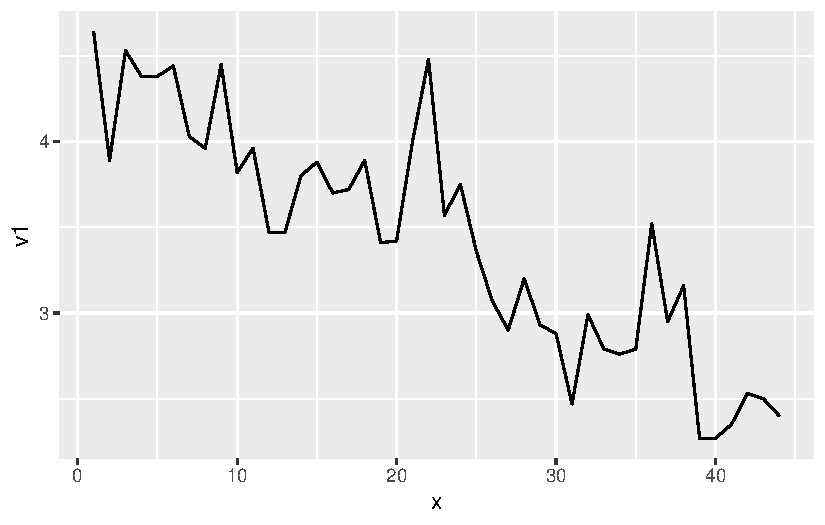
\includegraphics{MD_1_assignment_files/figure-pdf/unnamed-chunk-1-1.pdf}

}

\end{figure}

\begin{Shaded}
\begin{Highlighting}[]
  \FunctionTok{labs}\NormalTok{( }\AttributeTok{x =} \StringTok{"Season No."}\NormalTok{, }\AttributeTok{y =} \StringTok{"Views"}\NormalTok{)}
\end{Highlighting}
\end{Shaded}

\begin{verbatim}
$x
[1] "Season No."

$y
[1] "Views"

attr(,"class")
[1] "labels"
\end{verbatim}

\hypertarget{task-5}{%
\section{task 5}\label{task-5}}

\begin{Shaded}
\begin{Highlighting}[]
\FunctionTok{library}\NormalTok{(ggplot2)}
\NormalTok{viewers\_ep2 }\OtherTok{\textless{}{-}} \FunctionTok{c}\NormalTok{(}\FloatTok{3.47}\NormalTok{, }\FloatTok{3.80}\NormalTok{, }\FloatTok{3.88}\NormalTok{, }\FloatTok{3.70}\NormalTok{, }\FloatTok{3.72}\NormalTok{, }\FloatTok{3.89}\NormalTok{, }\FloatTok{3.41}\NormalTok{, }\FloatTok{3.42}\NormalTok{, }\FloatTok{4.00}\NormalTok{, }\FloatTok{4.48}\NormalTok{, }\FloatTok{3.57}\NormalTok{, }\FloatTok{3.75}\NormalTok{, }\FloatTok{3.36}\NormalTok{, }\FloatTok{3.07}\NormalTok{, }\FloatTok{2.90}\NormalTok{, }\FloatTok{3.20}\NormalTok{)}
\NormalTok{viewers\_ep3 }\OtherTok{\textless{}{-}} \FunctionTok{c}\NormalTok{(}\FloatTok{2.93}\NormalTok{, }\FloatTok{2.88}\NormalTok{, }\FloatTok{2.47}\NormalTok{, }\FloatTok{2.99}\NormalTok{, }\FloatTok{2.79}\NormalTok{, }\FloatTok{2.76}\NormalTok{, }\FloatTok{2.79}\NormalTok{, }\FloatTok{3.52}\NormalTok{, }\FloatTok{2.95}\NormalTok{, }\FloatTok{3.16}\NormalTok{, }\FloatTok{2.27}\NormalTok{, }\FloatTok{2.27}\NormalTok{, }\FloatTok{2.35}\NormalTok{, }\FloatTok{2.53}\NormalTok{, }\FloatTok{2.50}\NormalTok{, }\FloatTok{2.40}\NormalTok{)}
\NormalTok{df }\OtherTok{\textless{}{-}} \FunctionTok{data.frame}\NormalTok{(}\AttributeTok{x =} \DecValTok{1}\SpecialCharTok{:}\FunctionTok{length}\NormalTok{(viewers\_ep2), }\AttributeTok{v1 =}\NormalTok{ viewers\_ep3, }\AttributeTok{v2 =}\NormalTok{ viewers\_ep2)}
\FunctionTok{ggplot}\NormalTok{(}\AttributeTok{data =}\NormalTok{ df, }\FunctionTok{aes}\NormalTok{(}\AttributeTok{x =}\NormalTok{ x)) }\SpecialCharTok{+}
  \FunctionTok{geom\_line}\NormalTok{(}\FunctionTok{aes}\NormalTok{(}\AttributeTok{y =}\NormalTok{ v1)) }\SpecialCharTok{+}
  \FunctionTok{geom\_line}\NormalTok{(}\FunctionTok{aes}\NormalTok{(}\AttributeTok{y =}\NormalTok{ v2)) }\SpecialCharTok{+}
  \FunctionTok{labs}\NormalTok{(}\AttributeTok{title =} \StringTok{"Comparison"}\NormalTok{, }\AttributeTok{x =} \StringTok{"Season No."}\NormalTok{, }\AttributeTok{y =} \StringTok{"Views"}\NormalTok{)}
\end{Highlighting}
\end{Shaded}

\begin{figure}[H]

{\centering 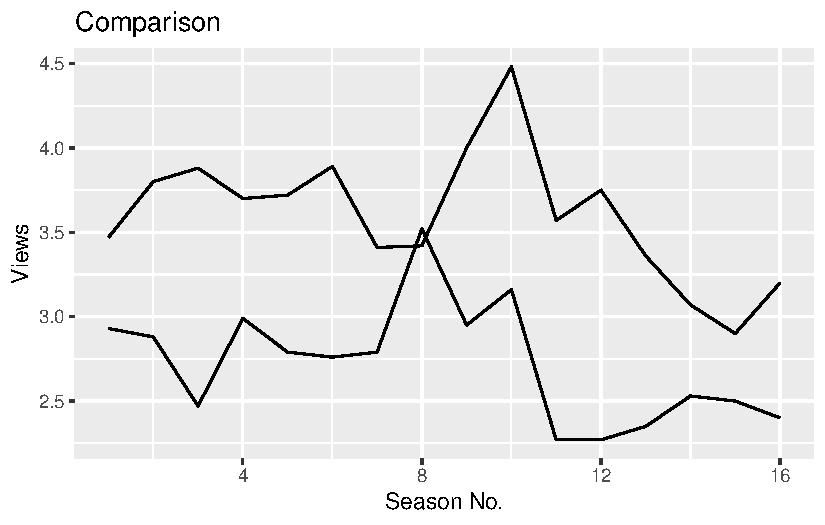
\includegraphics{MD_1_assignment_files/figure-pdf/unnamed-chunk-2-1.pdf}

}

\end{figure}



\end{document}
